\documentclass[letterpaper,11pt]{article}
\setlength{\textwidth}{6.5in}
\setlength{\hoffset}{0in}
%TODO: tweak these a bit more
\setlength{\voffset}{-0.5in}
\setlength{\textheight}{8.75in}
\setlength{\marginparsep}{0in}
\setlength{\marginparwidth}{0in}
\setlength{\oddsidemargin}{0in}

\usepackage{aas_macros}
\usepackage{amssymb}
\usepackage{hyperref}
\usepackage{listings}

\usepackage{graphicx}
\usepackage{lineno}
\usepackage[authoryear,square,colon]{natbib}
\bibpunct{[}{]}{;}{a}{,}{,~}

\begin{document}


\title{Determining the significance of associations between two series
of discrete events: bootstrap methods}
\author{J.~T. Niehof \and S.~K. Morley}
\date{\today}
\maketitle

\begin{abstract}
We review and develop techniques to determine associations between
series of discrete events. The bootstrap, a nonparametric statistical
method, allows the determination of the significance of associations
with minimal assumptions about the underlying processes. We find the
key requirement for this method: one of the series must be
widely spaced in time to guarantee the theoretical applicability of
the bootstrap. If this condition is met, the calculated signifance
passes a reasonableness test.  We conclude with some potential future
extensions and caveats on the applicability of these methods. The
techniques presented have been implemented in a Python-based software
toolkit.
\end{abstract}

%\linenumbers

\section{Introduction}
\label{sec:intro}
A question of frequent interest across many fields is the possible
relationship between two types of observation, potentially with some
time delay. Several familiar tools, such as regression analysis and
cross-correlations, relate continuously varying quantities. We expect,
for example, a strong correlation between the time series of
temperatures in White Rock and Los Alamos. A somewhat weaker
correlation would be evident between Los Alamos and Oklahoma
City, with Los Alamos expected to lag by about half an hour in the
dominant diurnal variation.

Less familiar are tools for associating point events, rather than
continuously varying quantities. For instance we may be interested in
a possible association between hailstorms in Los Alamos and work
requests at body shops in northern New Mexico. Although potentially
reducible to pseudo-continuous quantities (e.g., storms per month and
body shop jobs per month), this reduction loses the temporal
association between individual events and may require a period of
averaging longer than the delay between types of events. This report
reviews and extends techniques for determining the level of
association between two types of event, any delay in the association,
and a confidence that the observed level of association is significant
(beyond that expected from chance.) These techniques are agnostic
with respect to causality and work even if only a subset of each event
class is associated with the other: there may be reasons other than
hailstorms to seek body shop work. Subject to the caveats in
section~\ref{sec:ci}, they also work for clustered events,
e.g., multiple requests for body work following a single hailstorm.

This report builds on methods presented in the space sciences by
\citet{2007GeoRL..3408104M}, who examined the association between
magnetospheric substorms and ``trigger events'' in the upstream solar
wind. Python code implementing the methods of this report is available
in the LANL SpacePy package \citep[LA-CC-10-064;][]{spacepy11},
available under an open source license from
\url{http://spacepy.lanl.gov/}. These techniques are applicable to a
range of scientific studies.

\section{Review of techniques}
\subsection{Association analysis}
\label{sec:aa}
We are concerned with two time series of events, called series A and
series B throughout this manuscript. Each series is described by a
list of times when events of the appropriate type occurred. Each event
of type A is considered identical to all other type A events, and type
B events are similarly identical. We wish to determine whether events
of type B happen more frequently in some period of time before or
after events of type A; that is, whether there is some association
between series A and series B. \citet{cox55} developed these methods,
here called ``association analysis,'' relating textile defects to
halts of weaving machines. They were further developed by
\citet{brillinger76}, in the context of neuronal firing. Figures 1 and
2 of \citet{brillinger76} provide an excellent example of the
conversion from a continuously varying measurement to a series of
events. \citet{2007GeoRL..3408104M} provide another example:
converting from a time series of solar wind magnetic field
measurements to a list of ``trigger'' event times for one process, and
(implicitly) from a time series of various geomagnetic indicators to a
list of substorm times. The presentation here is after
\citet{2007GeoRL..3408104M}.

We consider a length of time $T$ in which we have measurements of a
series of $N_A$ type A events, where the $i^{th}$ event is denoted
$a_i$, and $N_B$ type B events, where the $j^{th}$ event is denoted
$b_j$. We assume a time lag $u$ between the series of events, and a
half-window $h$ representing an uncertainty in the timing of events or
in the delay between them. Then the $i^{th}$ individual association on
series A is defined:
\begin{equation}
\label{eq:assoc_number}
c_{A,i} = \#\{|b_j + u - a_i| < h\}
\end{equation}
where $\#\{\}$ is the number of events in set $\{\}$. In the zero-lag
case, this is the number of B events $b_j$ which fall within
half-window $h$ of a particular A event $a_i$. A non-zero lag has the
effect of time-shifting series B with respect to series
A. Figure~\ref{fig:series_example} presents a schematic example. Note
that, in this formulation, overlapping half-windows do not add to the
individual associations: one event must fall within the half-window of
the other.

\begin{figure}
\begin{center}
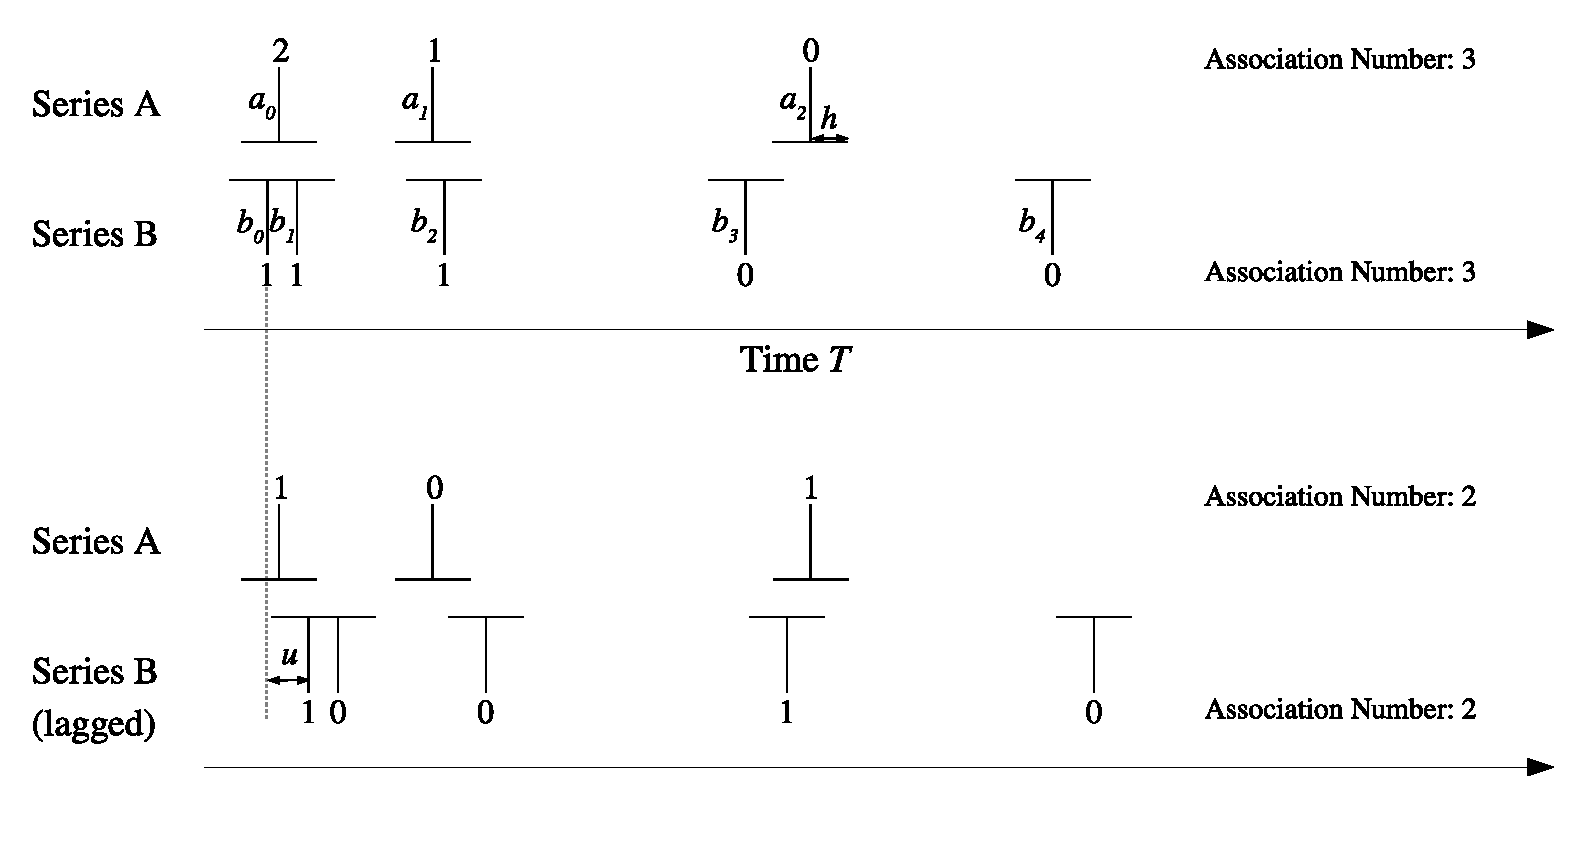
\includegraphics[width=0.75\textwidth]{figures/series_example.eps}
\caption{\label{fig:series_example}Two series of different types of
events (A and B), represented as vertical segments on a timeline
($a_i$, $b_j$).  Each event is labelled with its individual
association $c_{A,i}$ or $c_{B,j}$, the number of events of the other
type within a half-window $h$ of the event.  Top is the zero-lag case;
bottom, with series B shifted by lag $u$.}
\end{center}
\end{figure}

The total association number, usually just called the association
number, as a function of lag and half-window is:
\begin{equation}
\label{eq:assoc_total}
n(u, h) = \sum\limits_{i=1}^N c_{A,i}
\end{equation}
Note that the association number is independent of the choice of which
series is A and which is B (reversing the series simply reverses the
order of summation), but the individual associations $c$ are
not. Section~\ref{sec:ci} discusses the consequences of this
asymmetry. The association number can be viewed as ``the number of
occurrences where an A-type event and a B-type event are within a
half-window of each other'', where, e.g., two A events and two B events
all falling within a single half-window would result in four such
associations.

In practice we often have no a priori knowledge of the lag between
events, but wish to determine it. Thus the
association number is calculated by equation~\ref{eq:assoc_number} for
a large number of possible lags $u$ covering the expected range of
lags between the processes, a computationally intensive process which
nonetheless is tractable and even fast on modern computing
equipment. The half-window $h$ can also be optimized through a search
procedure (section~\ref{sec:window}).

\begin{figure}
\begin{center}
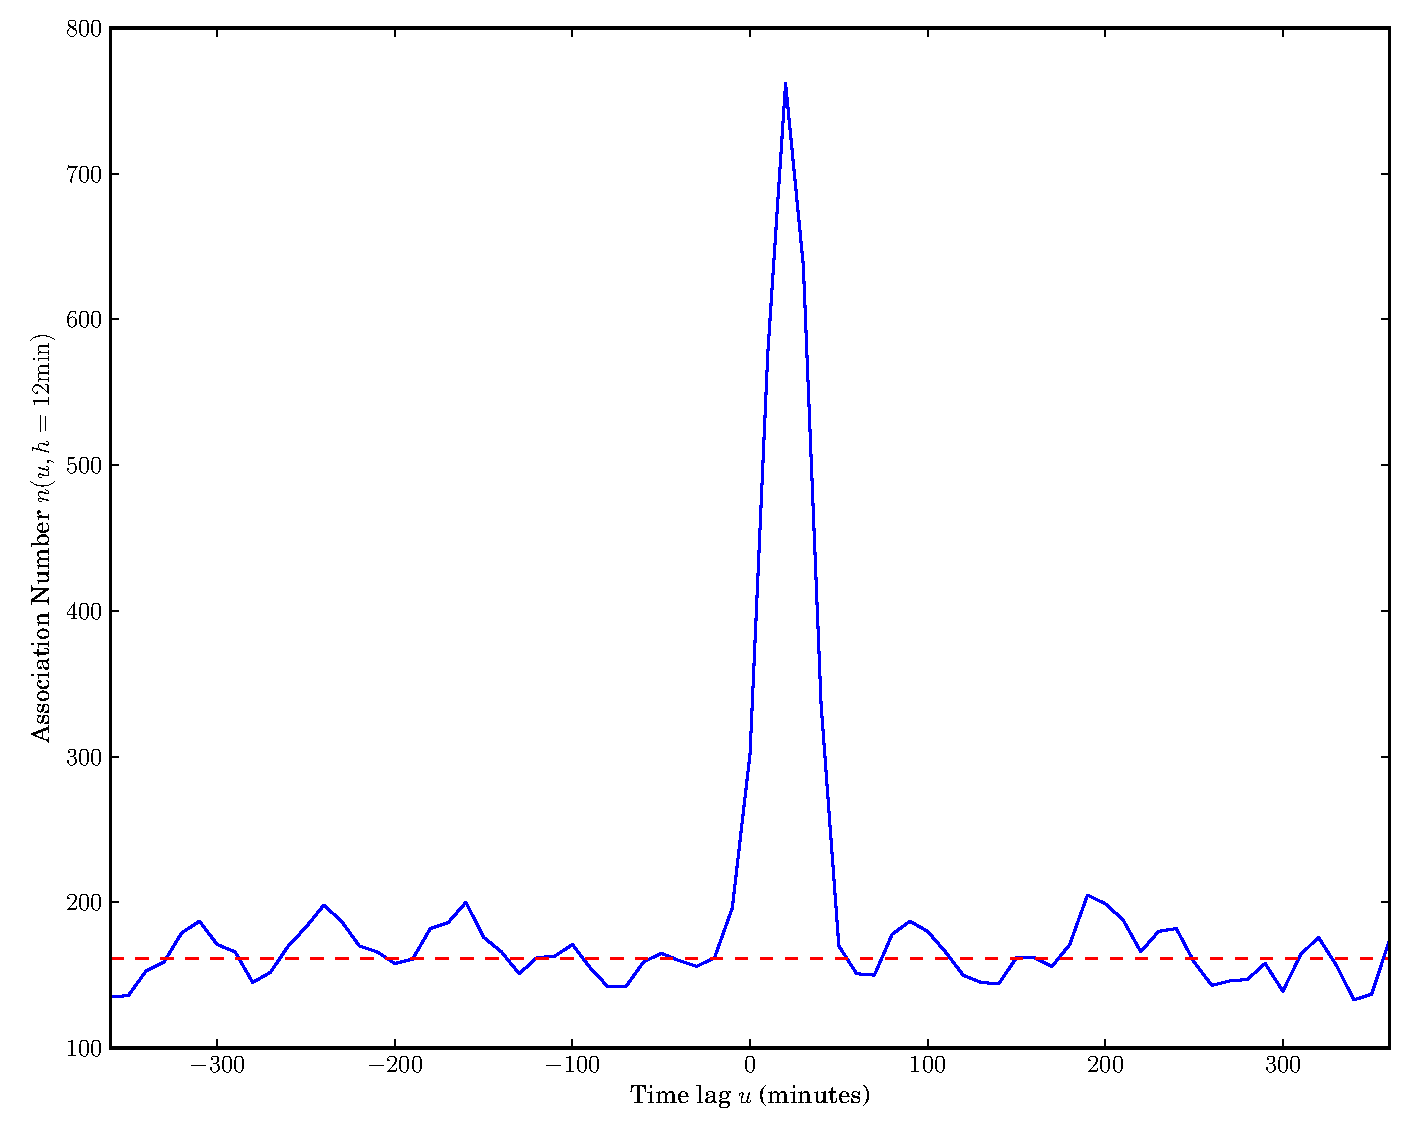
\includegraphics[width=0.75\textwidth]{figures/no_ci.eps}
\caption{\label{fig:assoc_only}Association number as a function of lag
for a synthetic example.}
\end{center}
\end{figure}

The result is a list of $n(u, h)$ generally plotted for a fixed $h$,
e.g., figure~\ref{fig:assoc_only} (produced by the PoPPy module of
SpacePy). This result is from a pair of synthetic series. Series A is
a series of 360 events whose times are determined by drawing from a
uniform random distribution on the interval [-90, 630] and using the
value as the event time (here given units of hours). Series B is a set
of 882 events for which the times were determined using a Gaussian
probability of occurrence around each event in series A, limited to
the interval [0, 540]. The peak of the Gaussian is 20 minutes after
the series A events, the half-width 10 min. Thus, as expected,
the association number increases around lags of 20 min., i.e., with
series A preceding series B by 20 min. The window half-width
for this analysis is 12 min.

Several methods can be used to distinguish ``real'' associations from
chance. The dotted red line in figure~\ref{fig:assoc_only} shows one
method. At very high lags, we expect any physical association between
the series to be broken. Thus the association number at these high
lags should tend to that of chance association; this is called the
aysmptotic association number $n(u\rightarrow\infty, h)$.
``Very high'' depends on the nature of the problem; in this
case, with a known 20 min. offset and half-width of 10 min.,
100 min. should suffice. The line plotted is the
median of the association numbers from the $0^{th}$ to $20^{th}$ percentile of
the lags and from the $80^{th}$ to $100^{th}$ percentile. This asymptotic
association number is about 162.  Association numbers
above this line indicate an association greater than chance; below, an
association less than chance, implying a reduction in occurrence of
one set of events at some lag relative to the other set. The
association analysis says nothing about causality: although the series
plotted shows an association between B events and A events 20
min. later, B does not necessarily cause A; some external process
may drive both. It would be unexpected for A to somehow cause B in
this instance.

An alternative means of finding the ``chance'' association number is
to examine the expected level of association if events were randomly
distributed \citep[cf.][]{brillinger76}. In this case, the probability
per unit time of a B event is:
\begin{equation}
\label{eq:prob_density}
p_B = \frac{N_B}{T}
\end{equation}
Then the number of type B events within a half-window $h$ is $2 h p_B
= \frac{2 h N_B}{T}$, and this number of events is expected to be
associated with each A event. The predicted total association number,
summing over all A events, is then:
\begin{equation}
\label{eq:total_predicted}
n_{expected}(u, h) = \frac{2 h N_A N_B}{T}
\end{equation}
For the pair of series presented, this evaluates to 166, close to the
asymptotic number of 162.

There are two subtleties to equation~\ref{eq:total_predicted}: first,
to justify equation~\ref{eq:prob_density}, B events must have a
constant probability over time and be independent of each other,
i.e., B must be essentially a Poisson process. As derived, there is no
such constraint on series A; thus, by the symmetry of the derivation,
either series A or B must be Poisson. Otherwise, the exact value of
$n_{expected}$ may be inaccurate, but we would still expect scaling
proportional to $N_A$, $N_B$, and $\frac{h}{T}$. The second subtlety
is an implicit $u$ dependence: as $u$ varies, the shifted series B may
not completely overlap with series A, and so in practice $N_A$, $N_B$,
and $T$ apply to the region of overlap, varying slightly with $u$. In
the extreme case where all events in series A occur well before any
event in series B, there are no events in the overlap and
$n_{expected}$ is zero.

In addition to the expected strong peak at 20 min.,
figure~\ref{fig:assoc_only} shows several minor peaks, e.g., at $u = 190$
min., implying a positive association. This lag is well into the
asymptotic region where no association is expected: clearly there is
``noise'' on the association number and not every peak is
significant. One approach to identifying significant peaks is to take
the asymptotic variability as the uncertainty and only identify peaks
of greater magnitude than those in the asymptotic region; this was
suggested by \citet{brillinger76}, who also computed more robust confidence
intervals based on the assumption of Poisson
processes. Section~\ref{sec:ci} computes confidence intervals for an
association analysis with much weaker requirements on the input
series, relying on a nonparametric statistical tool: the bootstrap.

\subsection{Bootstrapping}
\label{sec:boots}
Any set of measurements on a system represents a sample of a
population, and a metric derived from that sample represents an
estimate for that metric over the population. Knowledge of the range
of likely values for the metric on the population provides more
information than this single value.  Usually two assumptions are made
to infer the population statistics from the sample: first, the sample
is assumed to be representative of the population; second, the
distribution of the population is assumed (frequently Gaussian or
Poisson.) If there is no a priori reason to assume a
well-behaved population, most statistical methods are not
justified. These limitations are not always heeded in publications.

\citet{efron79} noted that, if the sample is truly representative of
the population, this is sufficient to reconstruct the population
statistics in a computationally intensive way. \citet{diaconis83}
provide a simple explanation of this
``bootstrapping'' process: given a sample of size $N$, randomly select
$N$ values from this sample with replacement to create a ``surrogate''
sample. By resampling with replacement, some values from the original
sample may appear multiple times in the surrogate; others may not
appear at all. Repeating this resampling many ($\gtrsim 10^{3}$) of
times, and each time calculating the desired metric from the
surrogate, will provide a sample of possible metrics that reflect the
statistics of the underlying population. Then, for example, the 95\%
confidence interval for the metric on the population can be
inferred from the 2.5$^{\mathrm{th}}$ percentile and
97.5$^{\mathrm{th}}$ percentile of the surrogate metrics.

As an example, consider the series 1, 2, 5, 5, 6. The sample mean is
3.8; what is the range of likely means for the population? The
standard deviation is 1.9, so assuming a normal population, the 95\%
confidence interval ($2\sigma$) for the population mean is 2.1 --
5.5. But the sample is clearly not normal, and we have no reason to
expect the population would be. Applying the bootstrap, two possible
surrogates are 1, 1, 5, 5, 5 (mean 3.4) and 1, 5, 5, 1, 6 (mean 3.6).
For a series of length $N$, with $N$ members of the series to
choose and $N$ possibilities for each, there are $N^N$ possible
surrogates, 3125 for this small sample. Generation of 1000
bootstrapped surrogates yields an estimated 95\% confidence interval
of 2.0--5.4.

The requirement of a representative sample is not sufficient for
a trustworthy bootstrap. \citet{singh81} strengthened the theoretical
justification for the bootstrap but demonstrated its failure for
dependent data: that is, where a value in a sequence has some
dependency on the preceding value or values. \citet{kunsch89} and
\citet{liu92} developed a modified version, the ``moving block
bootstrap'' (MBB), for dependent data.

The MBB works by resampling blocks of values in the sample, rather
than individual values. For a sample of size $N$, overlapping blocks
of $M$ samples each are taken, resulting in $N-M+1$ blocks, each
block shifted by one sample from the previous. These blocks are
resampled into a new surrogate series, and the desired metric
calculated on the surrogate. Multiple variations on the MBB have been
proposed to counter the obvious ``edge effects'' (the first and last
value of the sample only occur in one block each); \citet{lahiri03}
references several examples but demonstrates that the simple MBB
provides accuracy comparable to the more complicated
methods. \citet{lahiri03} also addresses the question of optimal block
size; a rule-of-thumb is that the block should be of
order $N^{\frac{1}{4}}$ to $N^{\frac{1}{3}}$, but far more involved
algorithms are available.

All bootstrap methods are oriented towards a single series of
values. The bootstrap function in SpacePy accepts such a series and
the function to apply to the surrogates, returning the requested
confidence interval and, if desired, the probability that the true
value is below some reference.  The following section adapts these
methods to association analysis, where there are two series of
discrete events occurring at a particular time, rather than with a
particular value.

\section{Confidence intervals for associations}
\label{sec:ci}
\begin{figure}
\begin{center}
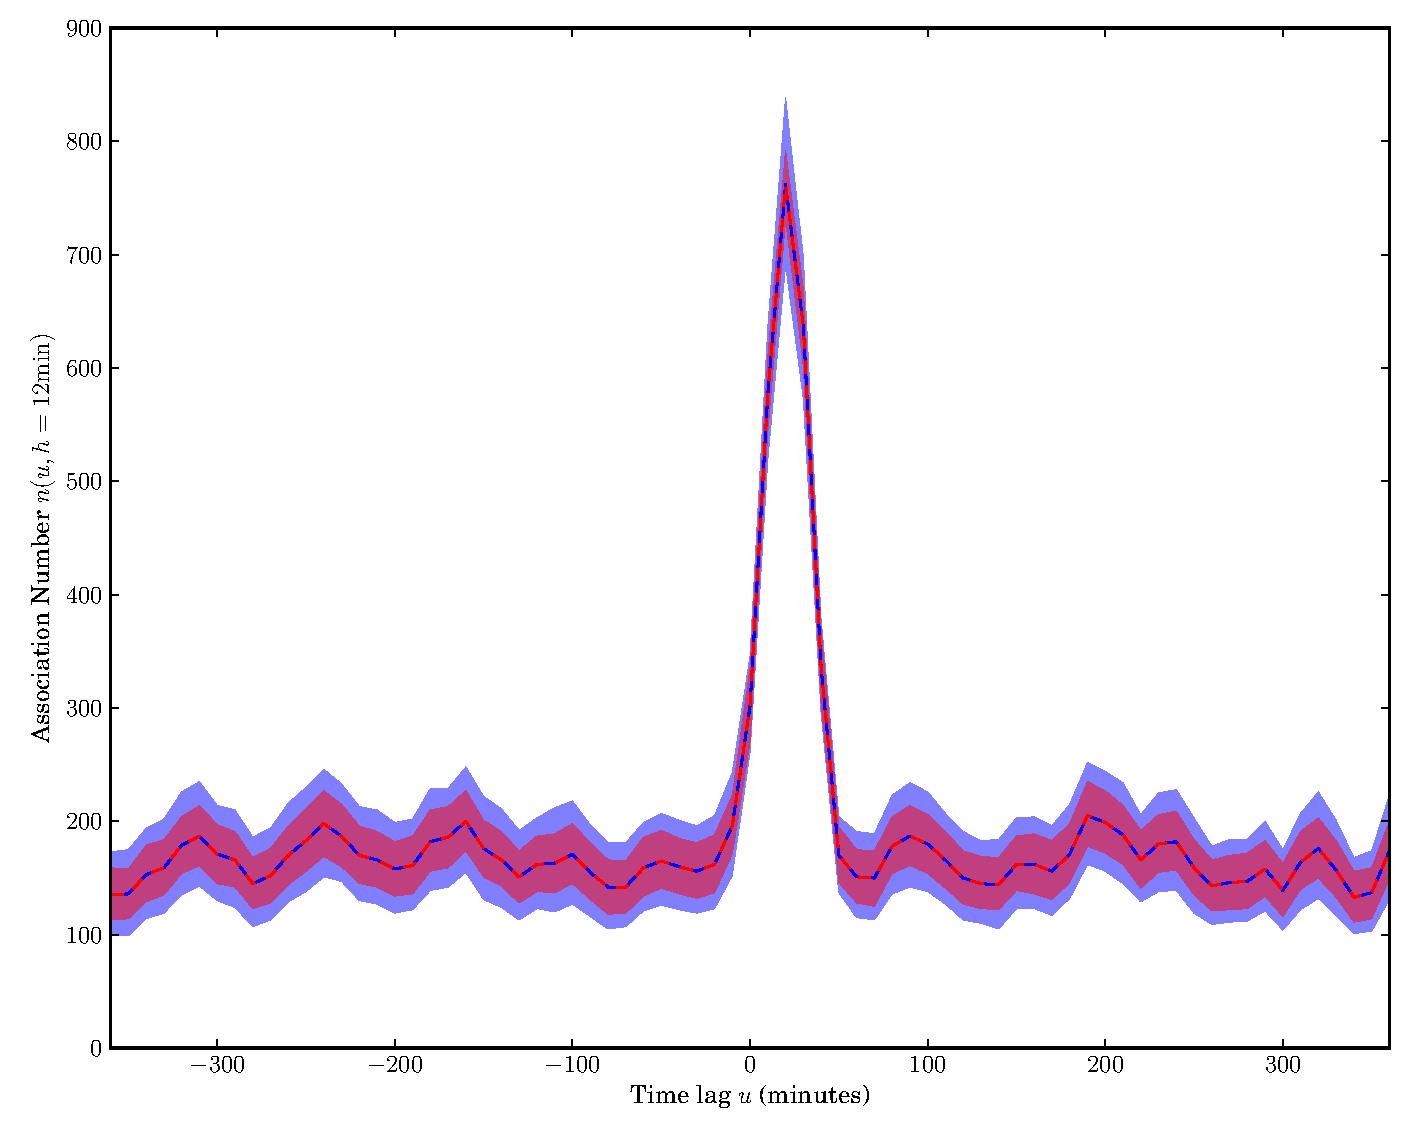
\includegraphics[width=0.75\textwidth]{figures/forward_vs_reverse.eps}
\caption{\label{fig:forward_reverse}Association number as a function
of lag, with 95\% confidence intervals. Blue line and blue fill are
association number and confidence interval based on calculating
individual associations for series A, then summing; red line and red
fill are based on summing over individual associations for series B.
Areas of overlapping confidence intervals are magenta.}
\end{center}
\end{figure}

\citet{2007GeoRL..3408104M} constructed bootstrap confidence intervals
on the association number by resampling the individual associations,
$c_{A,i}$ (equation~\ref{eq:assoc_number}), and evaluating the
appropriate percentiles of the sums across the surrogate series. This
approach breaks the symmetry between series A and B, as the series
$c_{A,i}$ is likely to be very different from $c_{B,j}$, although the
association numbers are the same. Figure~\ref{fig:forward_reverse}
shows the data of figure~\ref{fig:assoc_only} with 95\% confidence
intervals calculated over 4000 bootstrap iterations. The calculation
was performed twice: once as in figure~\ref{fig:assoc_only}, and once
with series A and B swapped. In the former case the bootstrap
resampled over the individual asociations for series A; in the latter,
over those for series B. For the calculation with swapped series, the
signs of the lags were inverted, as A leading B is equivalent to B
lagging A. It is clear that resampling over the 360 individual
associations for series A yielded more conservative confidence
intervals than resampling over the 882 series B individual
associations.

The question we wish to answer is symmetric: what is the probability
that the observed association is attributable to chance? The
confidence intervals based on association in one direction must be
more ``correct'' than the other, giving a better prediction for the
possible range of the population. It is tempting to ascribe the
tighter confidence interval when resampling over B to
$\frac{1}{\sqrt{N}}$ sampling effects, and indeed increasing the
density of events in series B without changing the distribution does
reduce the confidence interval. This only increases the disparity
between the confidence interval calculated by bootstrapping on series
A (which does not change) and bootstrapping on series B. Furthermore,
it is possible to create a pair of series such that bootstrapping on
the shorter series will result in a narrower confidence
interval. Clearly some means must be found to select the appropriate
series to bootstrap on.

\begin{figure}
\begin{center}
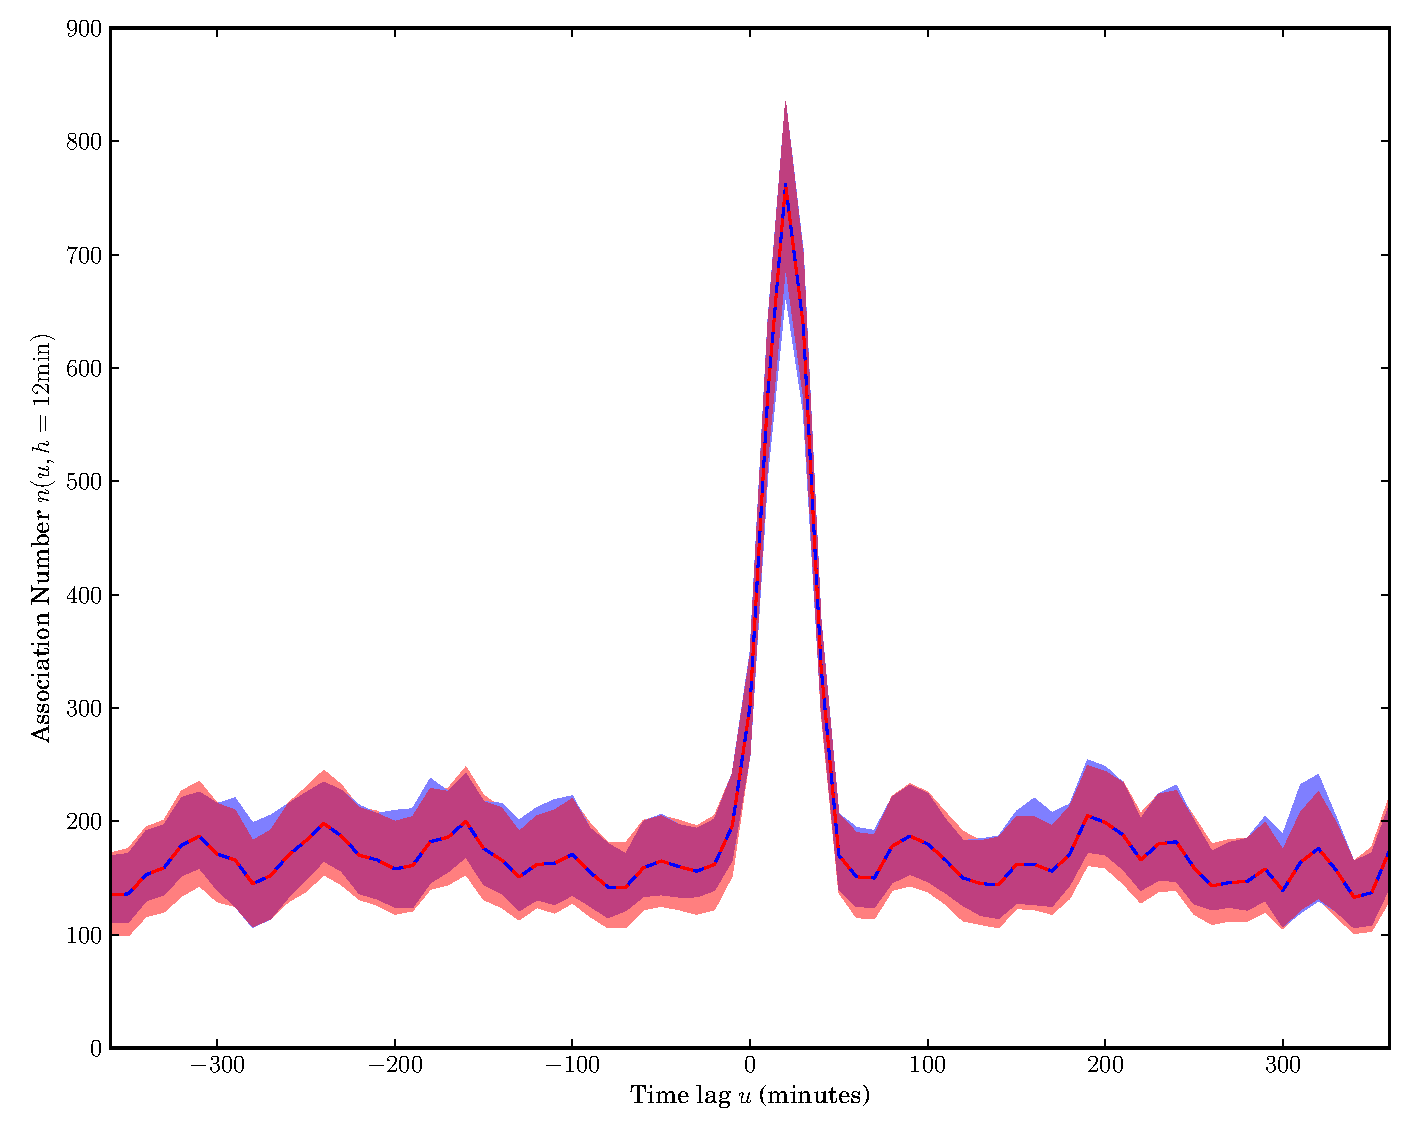
\includegraphics[width=0.75\textwidth]{figures/mbb_forward.eps}\\
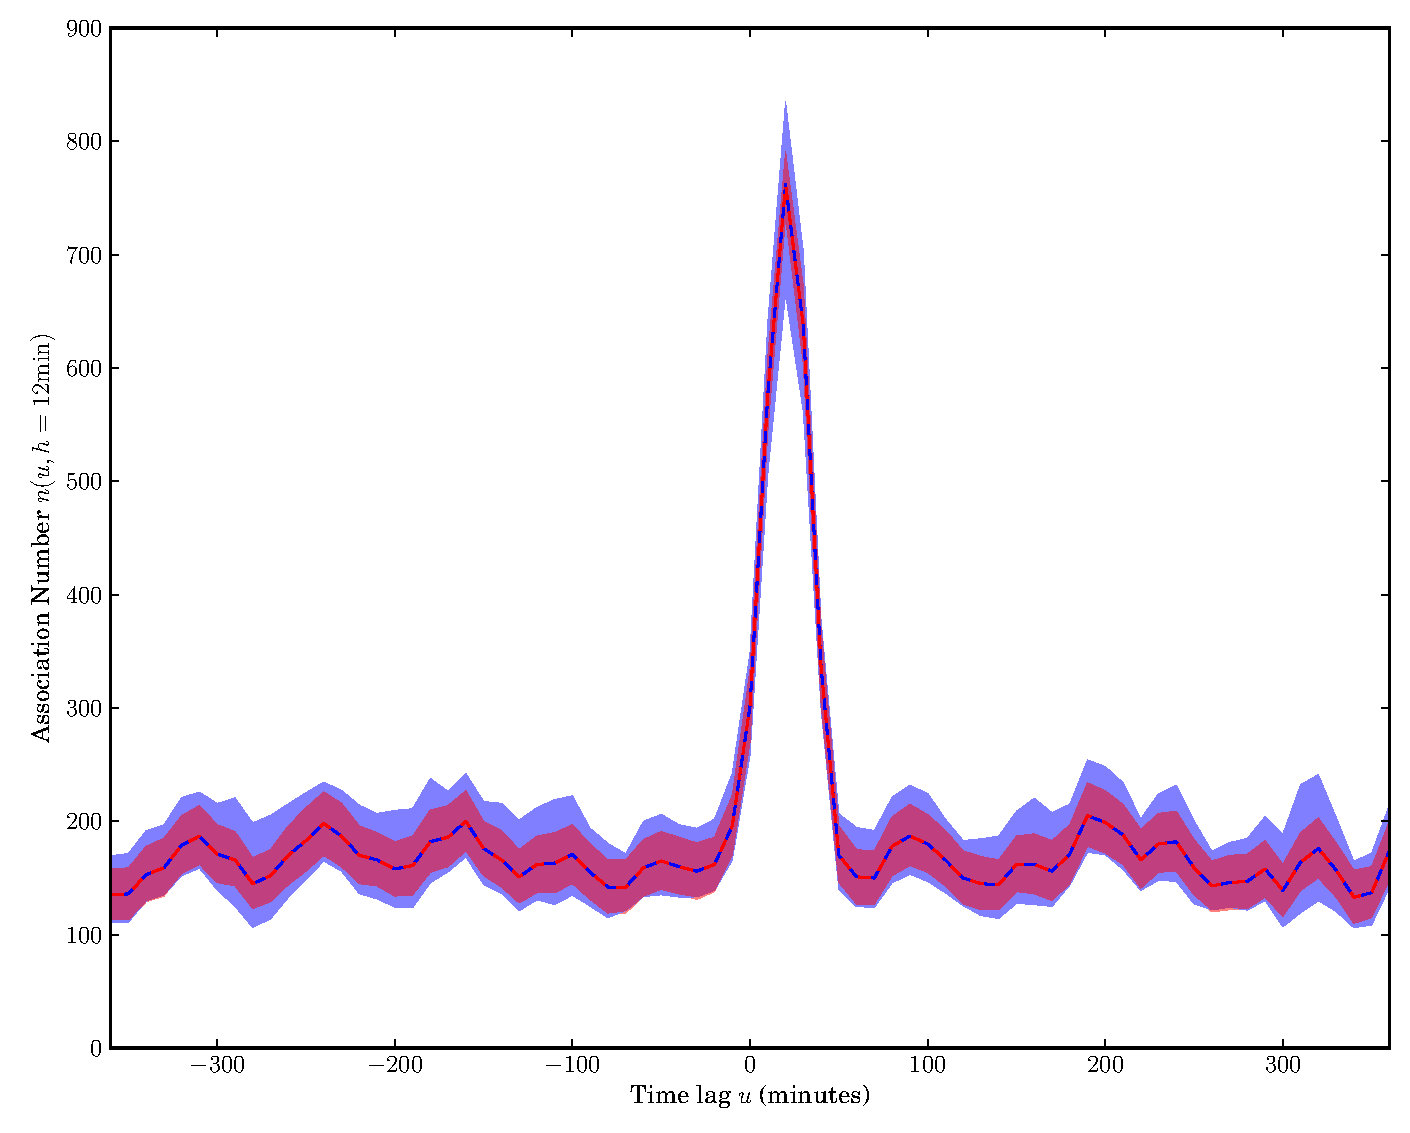
\includegraphics[width=0.75\textwidth]{figures/mbb_reverse.eps}
\caption{\label{fig:mbb_comparison}MBB 95\% confidence intervals, in
blue, compared to bootstrapping on the association number, in red;
overlap is in magneta. Top is in the ``forward'' sense, bottom in the
``backward'' sense.}
\end{center}
\end{figure}

Since the bootstrap requires the independence of individual values in
the sample, what if some dependence between events violates this
assumption? To test this possibility, we implemented a version of the
moving block bootstrap. The MBB defines a block as containing a
certain number of values from the sample. We chose to define a sample
as a single coincidence between series A and series B, with an
occurrence time halfway between the time of the series A event and the
(lagged) time of the series B event. Each block was then defined as a
period of time containing a certain number of coincidences, with block
boundaries halfway between coincidence times. Each block then had a
coincidence count $N_{A,B}$, time $T$, and counts of A, B events
$N_A$, $N_B$. Blocks were resampled with replacement to construct
surrogates, and totals of $N_{A,B}$, $T$, $N_A$, $N_B$ were computed
by summing over the blocks included in the surrogates. The number of
blocks in each surrogate was chosen to match the total $T$ to that of
the original series. $N_{A,B}$ for each surrogate was scaled by the
ratio of the expected value (equation~\ref{eq:total_predicted}) for
the original, nonresampled series to the expected value for the
resampled series. The confidence intervals from the resulting
bootstrap were completely symmetric when series A and B were swapped.

Figure~\ref{fig:mbb_comparison} shows the MBB-computed 95\% confidence
intervals after 4000 bootstrap iterations compared to the method of
figure~\ref{fig:forward_reverse}. The MBB has much better agreement
with bootstrapping over the series A individual associations than
bootstrapping over the series B associations, particularly at the
central peak. The MBB estimate appears to be somewhat asymmetric in
the asymptotic region, with the center of the 95\% confidence interval
at higher association numbers than the sample association number. In
the asymptotic region (absolute lags $>=120$ min.), the fraction of
the confidence interval above the calculated association number is
larger than the fraction below by 17\% (mean) to 18\% (median) of the
total confidence interval width. In contrast, asymmetries from
bootstrapping on the individual associations are of order
2\%--3\%. There are at least three possible reasons for this
offset. With low association numbers, there are few coincidences and
thus small blocksize and/or small number of blocks to bootstrap over,
and the sample may not be large enough to meet the bootstrap's
requirement that it be representative. It is also possible that the
requirement of blocks containing a certain number of coincidences
biases the estimate. Finally, this implementation of the MBB is based
on the expected association total, which lies in the interval
164.8--167.4 depending on the lag; the calculated asymptotic
association number (based on the median of largest lags, positive and
negative) is 161.7. Nonetheless, we can with reasonable confidence
conclude that bootstrapping over the series A association numbers
provides better confidence intervals than the series B association
numbers. This case mirrors that of \citet{2007GeoRL..3408104M} and
justifies their bootstrapping approach of modeling the sampling
variation in the individual associations.

\begin{table}
\begin{center}
\caption{ Comparison between association number 95\% c.i. and
asymptotic or expected values.\newline
{\footnotesize $n(u\rightarrow\infty)$ denotes comparison to the
asymptotic association number (section~\ref{sec:aa}) and
$n_{expected}$ to the expected association number
(equation~\ref{eq:total_predicted}). Restricted to high absolute lags
(120 min. or greater), where random variation should yield the
theoretical percentages within, below, and above the c.i.  Confidence
intervals calculated from surrogates of the series A individual
associations ($n*_{A}$), series B individual associations ($n*_{B}$),
or blocks generated by the moving block bootstrap ($n_{MBB}$).  Ranges
given are 95\% confidence interval for this percentage; see text }}
\label{table:ci_comparison}
\bigskip
\begin{tabular}{rr|ccc}
 & c.i. method & within c.i. & below c.i. & above c.i. \\
\hline
$n(u\rightarrow\infty)$ & $n*_{A}$ & 98\% (94--100) & 2\% (0--6) & 0\% \\
$n(u\rightarrow\infty)$ & $n*_{B}$ & 82\% (70--92) & 10\% (2--18) & 8\% (2--16)\\
$n(u\rightarrow\infty)$ & $n*_{MBB}$ & 92\% (84--98) & 8\% (2--16) & 0\% \\
$n_{expected}$ & $n*_{A}$ & 100\% & 0\% & 0\% \\
$n_{expected}$ & $n*_{B}$ & 82\% (70--92) & 8\% (2--16) & 10\% (2--18) \\
$n_{expected}$ & $n*_{MBB}$ & 92\% (84--98) & 6\% (0--14) & 2\% (0--6)\\
\multicolumn{2}{r|}{Theoretical} & 95\% & 2.5\% & 2.5\% \\
\end{tabular}

\end{center}
\end{table}

An additional check based on the definition of the confidence interval
can be made: in the asymptotic region, where variability is expected
to arise from chance, the asymptotic association number ($n(u\rightarrow\infty)$,
section~\ref{sec:aa}) should fall
within the 95\% confidence interval about 95\% of the time, below it
about 2.5\% of the time, and above it about 2.5\% of the time. For the
50 lags in the asymptotic region (absolute lags $>=120$ min.),
table~\ref{table:ci_comparison} shows what fraction of the association
numbers fell within the 95\% confidence interval, calculated from surrogates of the series A
individual associations ($n*_{A}$), series B individual associations
($n*_{B}$), or blocks generated by the moving block bootstrap
($n_{MBB}$). A similar comparison
is made for the expected association number at each lag
($n_{expected}$, equation~\ref{eq:total_predicted}). The ranges given are 95\%
confidence intervals, calculated by bootstrapping 40000 surrogates
from the asymptotic lags and finding the fractions for each
surrogate. This process gives, by definition, no knowledge of
uncertainty for the 100\% or 0\% case. These figures show that the MBB
asymmetry arises from a bias in this implementation, not a true
asymmetric confidence interval. Bootstrapping on the individual
associations shows no such bias, but bootstrapping over series B
yields confidence intervals which exclude the asymptotic (or expected)
number significantly more frequently than 95\%. We seek an explanation
why bootstrapping on series A should be more trustworthy.

The essential question for the applicability of the standard bootstrap
is the independence of samples, i.e. does the individual association
$c_{A,i}$ depend on the previous association $c_{A,i-1}$? If A-type
events are sufficiently separated in time, then no B event would be
associated with more than one A event, breaking any linkage between
the two. Indeed, the series were constructed to have wide spacing on
A: on average 120 hours between events compared to the analysis window
of 12 min. By contrast, the B events were selected to cluster
strongly around each A event. Thus the individual associations for B
events are not independent of each other, whereas the individual
associations for A events are independent. By the properties of the
bootstrap, then, bootstrapping on the independent A individual
associations should be more reliable, a choice confirmed by the above
analysis.

\section{Selection of window size}
\label{sec:window}
\begin{figure}
\begin{center}
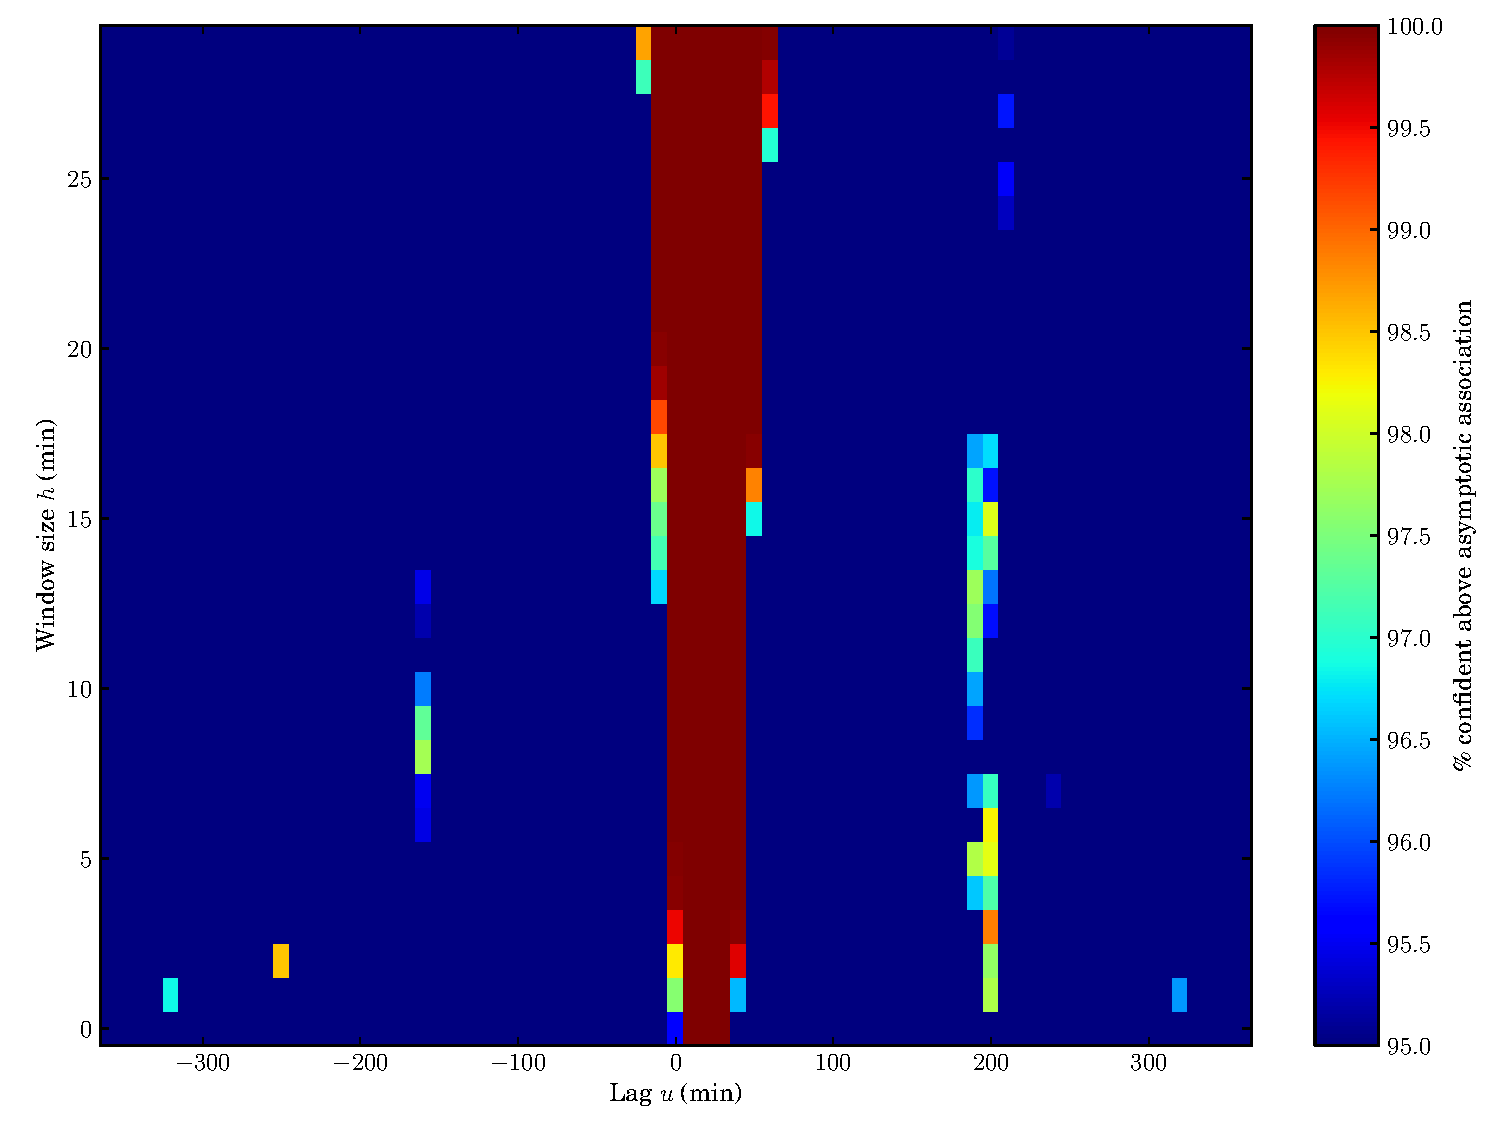
\includegraphics[width=0.75\textwidth]{figures/winsearch_conf.eps}
\caption{\label{fig:window_confidence}Confidence that the actual association
number is above the asymptotic association, as a function of lag and window
size.}
\end{center}
\end{figure}

\begin{figure}
\begin{center}
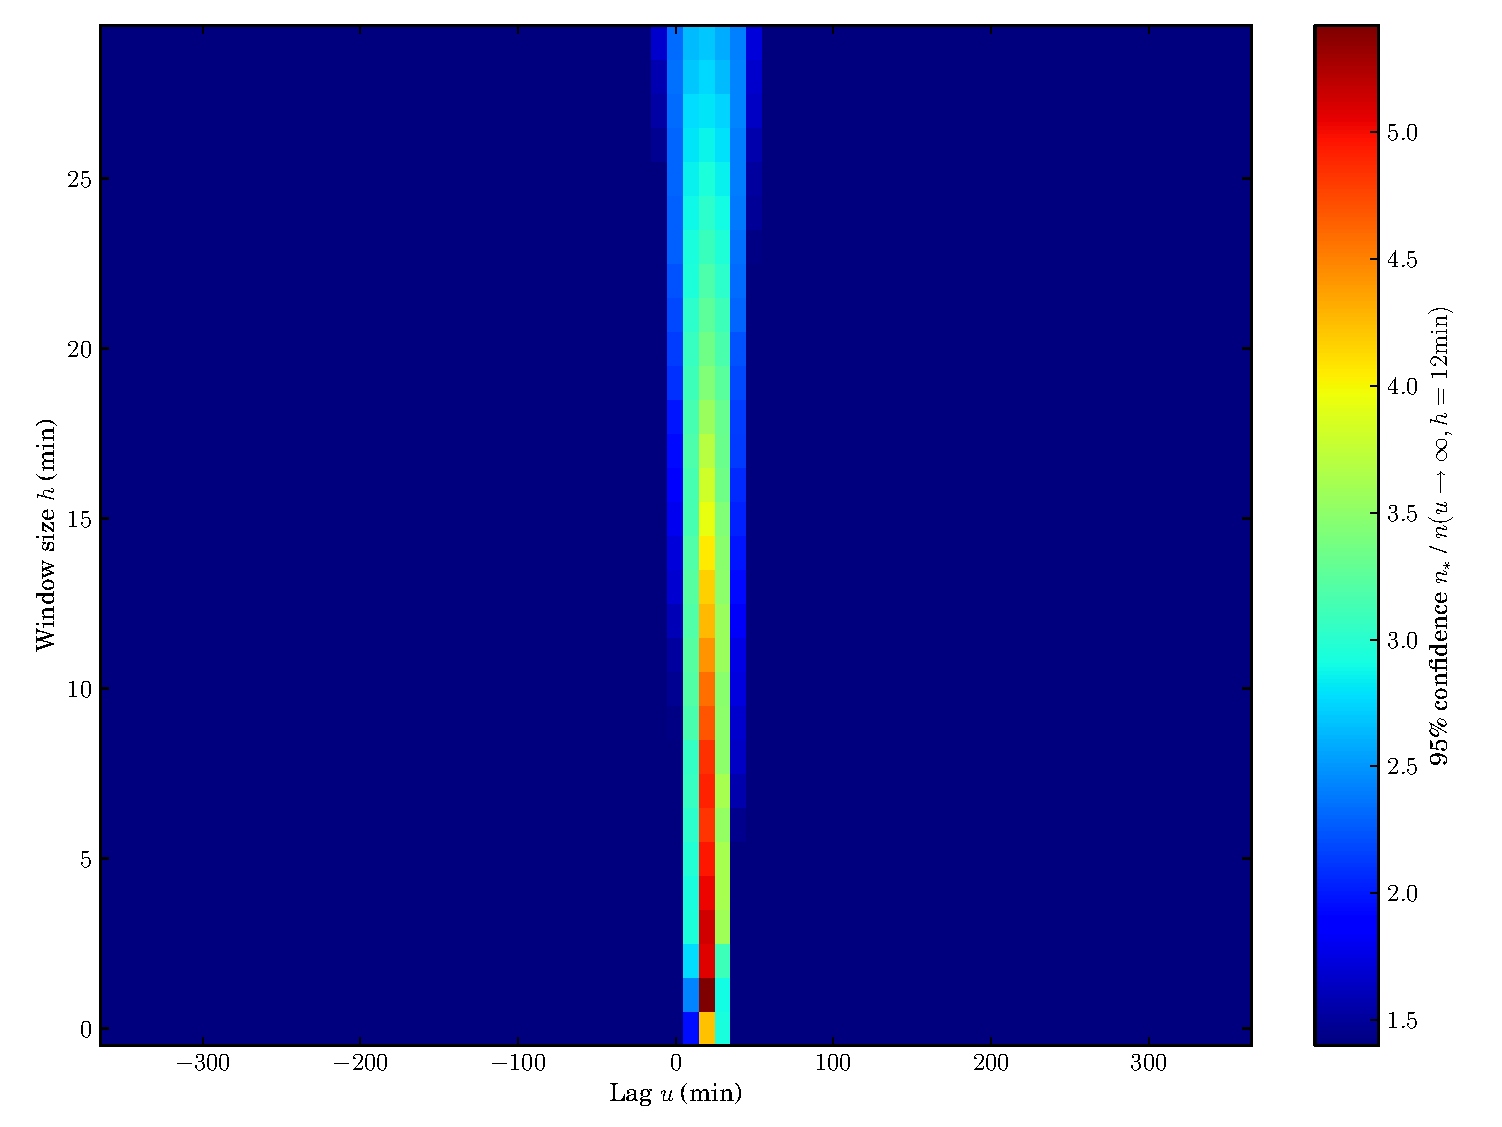
\includegraphics[width=0.75\textwidth]{figures/winsearch_ratio.eps}
\caption{\label{fig:window_ratio}Ratio of the calculated association
number's 95\% confidence interval lower limit to the asymptotic
association number, as a function of lag and window size.}
\end{center}
\end{figure}

The choice of window is somewhat arbitrary, although it can be
motivated by knowledge of uncertainties in timing or variability in
the response of the underlying system. An overly narrow window will
exclude real coincidences but provide sharper peaks in the association
number as a function of lag; an overly broad window will yield
uncertain estimates of the most significant
lag. \citet{2002JGRA..107.1398H} presented a graphical method of
searching for the optimal window size. They displayed the probability
of the association number being above the asymptotic number as a
function of both lag and window size, based on Poisson
statistics. This approach can be adapted to the bootstrap method, with
the results shown in figure~\ref{fig:window_confidence}. The peak at
20 min. lag is very apparent, and it is narrower for small window
sizes. The bootstrap requires the sample be representative of the
population, and there are few samples at the extrema of the
distribution, so it cannot determine significances close to 100\%. The
method (and the plot) saturates as a
result. Figure~\ref{fig:window_ratio} illustrates one approach to
finer-grained optimization of window size. Here the ratio of the
calculated association number to the upper 95\% confidence bound is
plotted, and the sharper peak at small window sizes is well
recovered. The method of figure~\ref{fig:window_confidence} provides a
first-cut minimum significance test, and figure~\ref{fig:window_ratio}
provides a means of maximizing the peak for windows meeting this
minimum test.

Just as knowledge of the system motivates the initial choice of
window, the optimal window size can be interpreted to infer some
underlying information. It may be indicative of a range of delays in
the process being measured; the width of the association peak is also
useful for this information.

It should be noted that if the data are used to define the best size
of search window, then the testing of the hypothesis should be
performed with a different, independent data set; defining the
hypothesis test using the data from which the hypothesis was
formulated artificially increases the likelihood of finding a
significant result.

\section{Future refinements}
\label{sec:future}
There are several potential enhancements to the techniques presented
in this report, which we intend to add to SpacePy.
\begin{itemize}
\item Bootstrapping on the individual associations is fast, simple,
and well-justified in certain cases, but a robust MBB implementation
would allow reliable association analysis in the case of
highly clustered events. In particular, a better implementation would
eliminate the biased confidence intervals shown in
figure~\ref{fig:mbb_comparison}.
\item Periodic or quasi-periodic signatures often appear in the
association number as a function of lag, extending into the asymptotic
region. Initial attempts to relate these periodicities to
periodicities on the input yielded mixed results. Properly filtering
these periodicities may allow the confident recovery of weaker
associations.
\item Speeding up the bootstrap would open up more areas of study. As
the association and bootstrapping code in SpacePy has evolved, we have
implemented significant speedups, but clever algorithms may improve
matters further. On modern machines with small enough data sets, the
possibility exists to calculate all possible surrogates
\citep{diaconis94a}, providing the best-possible bootstrap estimates
for a particular sample. For larger samples, it may be possible to
provide better coverage of the surrogate space with nonrandom
selection of properly ``spaced'' surrogates \citep{diaconis96},
similar to using Sobol sequences for other Monte Carlo problems. Where
a high level of certainty is required for a confidence interval at the
expense of the rest of the distribution, \citet{diaconis94b} presented
a method to focus bootstrap computations on the tails.
\end{itemize}

\section{Summary}
\label{sec:concl}
This report presents techniques for determining potential associations
between two types of event, a time lag in that association, and a
confidence that such association is beyond that expected from
chance. They are useful in a wide variety of applications. In the
sciences, they can be used to find connections and potential causality
between natural processes. They could also be used to evaluate the
effectiveness of intentional action: is an advertising campaign
associated with shoppers visiting a store? Is there a negative
association (decrease in the association number) between writing
speeding tickets and instances of speeding drivers? For how long does
this effect hold?

We examined several approaches for determining confidence intervals on
the association number. Bootstrapping on the individual associations
for one of the series provides reliable confidence intervals, provided
that the individual associations are independent of each other. This
requirement is fulfilled if that series has events widely separated in
time compared to the window half-width.

These powerful tools come with some caveats. As with all statistical
procedures, they require sufficient sampling to be
trustworthy. Appropriate confidence intervals are a guide, but the
bootstrap itself is not necessarily reliable for very small
samples. The elements of the series to which the bootstrap is applied
must be independent, unless a technique like the MBB is properly
applied. Applying any statistical tool indiscriminately in a hunt for
significance will likely mislead: performing 20 statistical tests
at 95\% confidence will normally discover a ``significant'' result
from simple chance. Finally, we include the standard caveat that
association neither proves nor implies causation: some third process
may drive both of the processes under investigation.

\appendix
\section{Code for the figures}
\label{sec:code}
Figures~\ref{fig:assoc_only}, \ref{fig:forward_reverse},
\ref{fig:window_confidence}, and \ref{fig:window_ratio} were produced
using the Point Processes in Python (PoPPy) module of SpacePy.
(Figure~\ref{fig:mbb_comparison} used experimental Moving Block
Bootstrap code, which has not been incorporated.) The code in this
appendix shows how to reproduce these plots. In the interest of
readability, cosmetic options (such as setting axis labels) have been
eliminated, as have commands to save the plots. This code requires
SpacePy, NumPy, and matplotlib.  \lstset{language=Python}
\begin{lstlisting}
import bisect
import math

from spacepy import poppy
import matplotlib
import matplotlib.pyplot as plt
import numpy

#Create the series
gauss = lambda x: math.exp(-(float(x - 20) ** 2) / (2 * 10 ** 2)) / \
        (10 * math.sqrt(2 * math.pi))
lags = range(-60 * 6, 60 * 6 + 1, 10) #minutes, up to quarter day
numpy.random.seed(1337)
series1 = numpy.random.randint(60 * -15 * 6, 60 * 105 * 6 + 1,
    [60 * 6])
series1.sort()
series1 = numpy.array(series1, dtype='float64')
randvals = numpy.random.rand(60 * 90 * 6 + 1)
series2 = numpy.fromiter((
    i for i in xrange(0, 60 * 90 * 6 + 1)
    if gauss(i - series1[bisect.bisect_right(series1, i) - 1]) + 
       gauss(i - series1[bisect.bisect_left(series1, i)])
       > 0.25 * randvals[i]
    ), numpy.float64, count=-1)

#Create a PPro object from the series
pop = poppy.PPro(series1, series2, lags=lags, winhalf=12.0)
pop.assoc() #Perform association analysis

#Figure 2
pop.plot(norm=False)

pop.aa_ci(95, n_boots=4000) #Generate confidence intervals

#Do the same for the series in the reverse order
poprev = poppy.PPro(series2, series1, lags=lags[-1::-1], winhalf=12.0)
poprev.assoc()
poprev.aa_ci(95, n_boots=4000)
poprev.lags = lags

#Figure 3
poppy.plot_two_ppro(pop, poprev, ratio=1.0)
plt.show() 

#Set up for window search algorithm
pop_2d = poppy.PPro(series1, series2, lags=lags, winhalf=12.0)
windows = numpy.array(range(30), dtype='float64')
(low, high, percentile) = pop_2d.assoc_mult(windows, n_boots=10000,
                          seed=1337)

#Figure 5
pop_2d.plot_mult(windows, percentile, min=95.0)
plt.show()

#Figure asymptotic association for all windows
asymptotes = numpy.empty([30], dtype='float64')
for i in range(len(windows)):
    junk = poppy.PPro(series1, series2, lags=lags, winhalf=windows[i])
    junk.assoc(h=windows[i])
    asymptotes[i] = junk.asympt_assoc

#Ratio of bottom of c.i. to asymptote
ratios = numpy.empty(low.shape, dtype='float64')
for i in range(len(windows)):
    ratios[i, :] = low[i, :] / asymptotes[i]

#Figure 6
pop_2d.plot_mult(windows, ratios, min=1.4,
                 cbar_label=r'95 percent confidence / asymptote')
plt.show()
\end{lstlisting}

\section{The bootstrap function in SpacePy}
\label{sec:boots_ci}
The \texttt{aa\_ci} method of \texttt{PPro} objects selects surrogates
from the individual associations and sums each surrogate series to
find association numbers based on the surrogates, determining the 95\%
confidence interval from the $\mathrm{2.5^{th}}$ and
$\mathrm{97.5^{th}}$ percentile of the surrogate association
numbers. The underlying function, \texttt{boots\_ci}, is available for
more general use. It requires a sequence from which to select
surrogates, the number of surrogate series to produce, a desired
confidence interval, and any Python function which can be applied to a
series for the desired metric. The following code implements the
example of section~\ref{sec:boots}.
\begin{lstlisting}
import numpy
from spacepy import poppy

seq = [1.0, 2.0, 5.0, 5.0, 6.0]
#numpy.mean and numpy.median find mean and media of a sequence
print(numpy.mean(seq))
print(numpy.median(seq))

#Find 95 percent confidence intervals on mean, median
#Select 10000 surrogates
(lo, hi) = poppy.boots_ci(seq, 10000, 95, numpy.mean)
print('c.i. ' + str(lo) + ' through ' + str(hi))
print(poppy.boots_ci(seq, 10000, 95, numpy.median))

#What is the probability that the mean is above 4?
(lo, hi, prob) = poppy.boots_ci(seq, 10000, 95, numpy.mean, target=4.0)
print(str(prob) + ' percent chance mean greater than 4.')
\end{lstlisting}
The Python interface is backed by a fast C-based implementation, which
takes full advantage of modern multicore and multiprocessor machines.

\bibliographystyle{2011_assoc}
\bibliography{2011_assoc}

\end{document}

